\chapter{Multivariate Functions, Limit and Continuity}
\lecture{8}{21 May. 23:18}{Eight Lecture}
\label{chap:multivariate-functions}

\section{Functions with Several Variables}
\label{sec:functions-with-several-variables}

\begin{definition}[Multivarite Function]
  \label{def:multivariate-function}
  Suppose \(D\) is a set of \(n\)-tuples of real numbers
  \((x_1,x_2,\ldots,x_{n})\). A \textbf{real-valued function} \(f\) on \(D\) is
  a rule that assigns a unique (single) real number 
  \[ w = f(x_1,x_2,\ldots,x_{n}) \]
  to each element in \(D\). The set \(D\) is the function's domain. The set of
  \(w\)-values take on by \(f\) is the function's range. The symbol \(w\) is
  the dependent variable of \(f\), and \(f\) is said to be a function of the
  \(n\) independent variables \(x_1\) to \(x_{n}\). We also call the
  \(x_{j}\)'s the function's input variables and call \(w\) the function's
  output variable.

  \begin{figure}[H]
    \centering
    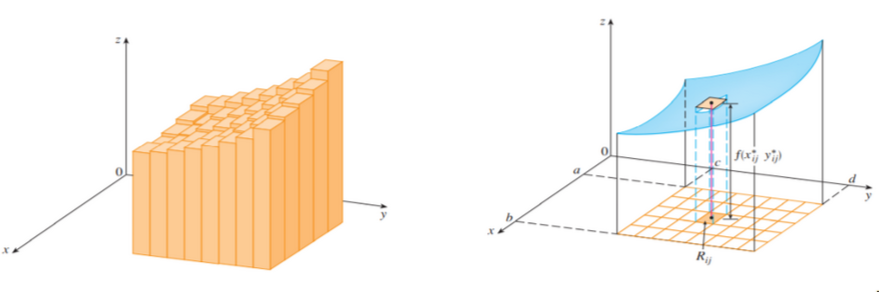
\includegraphics[width=0.8\textwidth]{Figures/pimg2.png}
    \caption{Multivarite Function}
    \label{fig:pimg4-multivarite-function}
  \end{figure}
\end{definition}

\section{Level Curve and Surface}
\label{sec:level-curve-and-surface}

\begin{definition}[Level Curve]
  \label{def:level-curve}
  The set of points in the plane where a function \(f(x,y)\) has a constant
  value \(f(x,y)=c\) is called a level curve of \(f\). The set of all points
  \((x,y,f(x,y))\) in space, for \((x,y)\) in the domain of \(f\), is called
  the \textbf{graph} of \(f\). The graph of \(f\) is also called the
  \textbf{surface \(z=f(x,y)\)}. 
  \begin{eg}
    \textbf{Graph \(f(x,y)=100-x^2-y^2\) and plot the level curves
      \(f(x,y)=0\), \(f(x,y)=51\), and \(f(x,y)=75\) in the domain of \(f\) in
    the plane.}
    \begin{figure}[H]
      \centering
      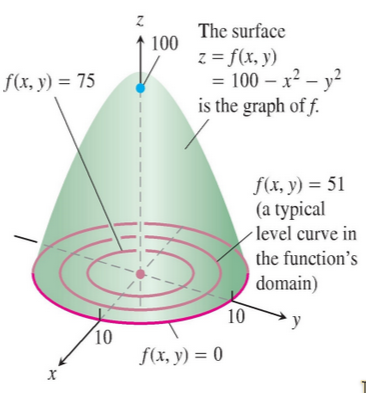
\includegraphics[width=0.8\textwidth]{Figures/pimg3.png}
      \caption{The graph and selected level curve of the function \(f(x,y)\)}
      \label{fig:level-curve}
    \end{figure}
  \end{eg}
\end{definition}

\begin{definition}[Level Surface]
  \label{def:level-surface}
  The set of points \((x, y, z)\) in space where a function of three
  independent variables has a constant value \(f(x, y, z) = c\) is called
  level surface of \(f\).
\end{definition}

\section{Limits in Higher Dimensions}
\label{sec:limits-in-higher-dimensions}

\begin{definition}[Limit]
  \label{def:limit-higher-dim}
  We say that a function \(f(x,,y)\) approaches the \textbf{limit} \(L\) as
  \((x,y)\) approaches \((x_o, y_o)\), and write:
  \[ \lim_{(x,y) \to (x_o,y_o)} f(x,y) = L \]
  \(\forall\ (x,y) \in \text{Domain}(f)\):
  \[
    \forall\ \epsilon>0, \exists \delta>0\\ 
    \implies 
    ( \sqrt{(x-x_{o})^2+(y-y_o)^2} <\delta 
    \implies  \left| f(x,y)-L \right| <\epsilon )
  \]. 

  \begin{figure}[H]
    \centering
    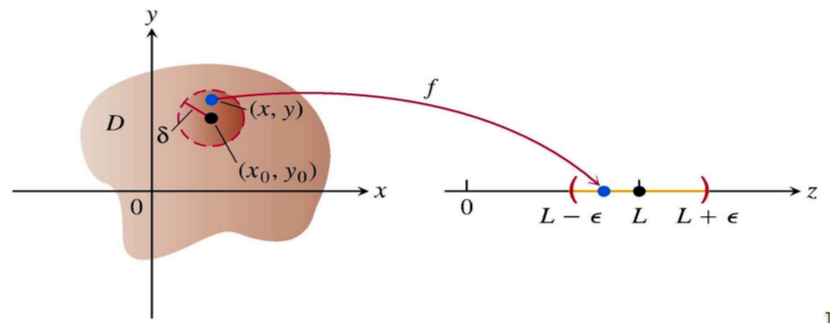
\includegraphics[width=0.8\textwidth]{Figures/pimg4.png}
    \caption{In the limit definition, \(\delta\) is the radius of a disk
      centered at \((x_o,y_o)\). \(\forall\) \((x,y)\) withint this disk, the
      function values \(f(x,y)\) lie inside the corresponding interval
    \((L-\epsilon,L+\epsilon)\)}
    \label{fig:limit-higher-dim}
  \end{figure}
\end{definition}

\begin{theorem}
  The following rules hold if \( L, M, \) and \( k \) are real numbers and
  \[
    \lim_{(x, y) \to (x_0, y_0)} f(x, y) = L \quad \text{and} \quad \lim_{(x, y) \to (x_0, y_0)} g(x, y) = M.
  \]
  \begin{enumerate}
    \item \textbf{Sum Rule:} \\
      \[
        \lim_{(x, y) \to (x_0, y_0)} [f(x, y) + g(x, y)] = L + M
      \]

    \item \textbf{Difference Rule:} \\
      \[
        \lim_{(x, y) \to (x_0, y_0)} [f(x, y) - g(x, y)] = L - M
      \]

    \item \textbf{Constant Multiple Rule:} \\
      \[
        \lim_{(x, y) \to (x_0, y_0)} kf(x, y) = kL \quad \text{(any number \( k \))}
      \]

    \item \textbf{Product Rule:} \\
      \[
        \lim_{(x, y) \to (x_0, y_0)} [f(x, y) \cdot g(x, y)] = L \cdot M
      \]

    \item \textbf{Quotient Rule:} \\
      \[
        \lim_{(x, y) \to (x_0, y_0)} \frac{f(x, y)}{g(x, y)} = \frac{L}{M}, \quad M \ne 0
      \]

    \item \textbf{Power Rule:} \\
      \[
        \lim_{(x, y) \to (x_0, y_0)} [f(x, y)]^n = L^n, \quad n \text{ a positive integer}
      \]

    \item \textbf{Root Rule:} \\
      \[
        \lim_{(x, y) \to (x_0, y_0)} \sqrt[n]{f(x, y)} = \sqrt[n]{L} = L^{1/n},
        \quad
      \]
      \(n\) a \(+\)ve integer, and if \( n \) is even,
      assume that  \(L > 0\).
  \end{enumerate}
\end{theorem}

\section{Continuity of a Multivarite Function}
\label{sec:continuity-of-a-multivarite-function}

\begin{definition}[Continuity of a Multivarite Function]
  \label{def:continuity-of-a-multivarite-function}
  A function \( f(x, y) \) is continuous at the point \( (x_0, y_0) \) if
  \begin{enumerate}
    \item \( f \) is defined at \( (x_0, y_0) \)
    \item \( \displaystyle \lim_{(x,y) \to (x_0,y_0)} f(x,y) \) exists.
    \item \( \displaystyle \lim_{(x,y) \to (x_0,y_0)} f(x,y) = f(x_0, y_0) \)
  \end{enumerate}

  A function is continuous if it is continuous at every point of the domain.
\end{definition}

\subsection{Two Path Test for Non-existence of a Limit}
\label{ssec:two-path-test-for-non-existence-of-a-limit}

If a function \( f(x,y) \) has different limits along two different paths in the domain of \( f \) as \( (x,y) \) approaches \( (x_0,y_0) \), then
\[
  \lim_{(x,y) \to (x_0,y_0)} f(x,y)
\]
does not exist.

\begin{remark}
  It is easy to prove non-existence of a limit rather that existence.
  \begin{eg}
    Show that:
    \[ 
      f(x,y)=
      \begin{cases}
        \frac{2xy}{x^2+y^2}&(x,y)\neq (0,0)\\
        0&(x,y)=(0,0)
      \end{cases}
    \] 
    is not continuos at origin.
  \end{eg}
  \begin{answer}
    \textbf{Along the path \(y=mx\)},
    \begin{align}
      \lim_{(x,y) \to (0,0)} f(x,y)
    &=\lim_{(x,y) \to (0,0)} \frac{2x.mk}{x^2+(mx)^2}\\
    &=\frac{2m}{1+m^2}
    \end{align}

    For \(k=1\) i.e, along the path \(y=x\), the limit is 1 and for \(k=-1\),
    the limit is \(-1\).

    \emph{So by two path test, limit of \(f(x,y)\) does not exist at origin.}
    \(\therefore\) The function is not continuous at origin through \(f(0,0)=0\)
  \end{answer}
\end{remark}

